\documentclass[10pt]{beamer}

\usetheme[progressbar=frametitle]{metropolis}

\usepackage{booktabs}
\usepackage[scale=2]{ccicons}


\usepackage{amsmath}
\usepackage{pgfplots}
\usepgfplotslibrary{dateplot}

\usepackage{xspace}
\newcommand{\themename}{\textbf{\textsc{metropolis}}\xspace}

%\usepackage{placeins} %%%
\usepackage{subfig}
\usepackage{physics}
\usepackage{amssymb}


\usepackage{tikz}
\usepackage{circuitikz}
\usepackage{siunitx}


\usepackage{latexsym}
\usepackage{mathtools}
\usepackage{slashed} % for the Feynman slash notation

\usepackage{listings}

\usepackage{balance}


% edited by Mauro 28-12-16
%
%% <local definitions>
\newcommand{\R}{\mathbb{R}}	
\newcommand{\C}{\mathbb{C}}
\newcommand{\HQ}{\mathbb{H}}
\newcommand{\N}{\mathbb{N}}
\newcommand{\be}{\begin{equation}}
\newcommand{\ee}{\end{equation}}	
\newcommand{\bea}{\begin{eqnarray}}
\newcommand{\eea}{\end{eqnarray}}	
\newcommand{\Pin}{\mathrm{Pin}}	
\newcommand{\Spin}{\mathrm{Spin}}
\renewcommand{\O}{\mathrm{O}}
\newcommand{\SO}{\mathrm{SO}}
\renewcommand{\eqref}[1]{(\ref{#1})}
\newcommand{\cl}[1]{\ensuremath{Cl(#1)}} % #1 stands for the values p,q. $\cl{p,q}$ produces 'Cl(p,q)'.
\newcommand{\gvec}[1]{\ensuremath{\mbox{\textbf{\textit{#1}}}}}
\newcommand{\vect}[1]{\ensuremath{\mbox{\textbf{\textit{#1}}}}}
%% </local definitions>

\newcommand{\Ba}[0]{\mathbf{a}}
\newcommand{\Bb}[0]{\mathbf{b}}
\newcommand{\Bc}[0]{\mathbf{c}}
\newcommand{\Bd}[0]{\mathbf{d}}
\newcommand{\Be}[0]{\mathbf{e}}
\newcommand{\Bf}[0]{\mathbf{f}}
\newcommand{\Bg}[0]{\mathbf{g}}
\newcommand{\Bh}[0]{\mathbf{h}}
\newcommand{\Bi}[0]{\mathbf{i}}
\newcommand{\Bj}[0]{\mathbf{j}}
\newcommand{\Bk}[0]{\mathbf{k}}
\newcommand{\Bl}[0]{\mathbf{l}}
\newcommand{\Bm}[0]{\mathbf{m}}
\newcommand{\Bn}[0]{\mathbf{n}}
\newcommand{\Bo}[0]{\mathbf{o}}
\newcommand{\Bp}[0]{\mathbf{p}}
\newcommand{\Bq}[0]{\mathbf{q}}
\newcommand{\Br}[0]{\mathbf{r}}
\newcommand{\Bs}[0]{\mathbf{s}}
\newcommand{\Bt}[0]{\mathbf{t}}
\newcommand{\Bu}[0]{\mathbf{u}}
\newcommand{\Bv}[0]{\mathbf{v}}
\newcommand{\Bw}[0]{\mathbf{w}}
\newcommand{\Bx}[0]{\mathbf{x}}
\newcommand{\By}[0]{\mathbf{y}}
\newcommand{\Bz}[0]{\mathbf{z}}
\newcommand{\BA}[0]{\mathbf{A}}
\newcommand{\BB}[0]{\mathbf{B}}
\newcommand{\BC}[0]{\mathbf{C}}
\newcommand{\BD}[0]{\mathbf{D}}
\newcommand{\BE}[0]{\mathbf{E}}
\newcommand{\BF}[0]{\mathbf{F}}
\newcommand{\BG}[0]{\mathbf{G}}
\newcommand{\BH}[0]{\mathbf{H}}
\newcommand{\BI}[0]{\mathbf{I}}
\newcommand{\BJ}[0]{\mathbf{J}}
\newcommand{\BK}[0]{\mathbf{K}}
\newcommand{\BL}[0]{\mathbf{L}}
\newcommand{\BM}[0]{\mathbf{M}}
\newcommand{\BN}[0]{\mathbf{N}}
\newcommand{\BO}[0]{\mathbf{O}}
\newcommand{\BP}[0]{\mathbf{P}}
\newcommand{\BQ}[0]{\mathbf{Q}}
\newcommand{\BR}[0]{\mathbf{R}}
\newcommand{\BS}[0]{\mathbf{S}}
\newcommand{\BT}[0]{\mathbf{T}}
\newcommand{\BU}[0]{\mathbf{U}}
\newcommand{\BV}[0]{\mathbf{V}}
\newcommand{\BW}[0]{\mathbf{W}}
\newcommand{\BX}[0]{\mathbf{X}}
\newcommand{\BY}[0]{\mathbf{Y}}
\newcommand{\BZ}[0]{\mathbf{Z}}

\newcommand{\ta}[0]{\tilde{a}}
\newcommand{\tb}[0]{\tilde{b}}
\newcommand{\tc}[0]{\tilde{c}}
\newcommand{\td}[0]{\tilde{d}}

\newcommand{\hA}[0]{\hat{A}}
\newcommand{\hB}[0]{\hat{B}}
\newcommand{\hH}[0]{\hat{H}}

\newcommand{\tA}[0]{\tilde{A}}
\newcommand{\tB}[0]{\tilde{B}}
\newcommand{\tF}[0]{\tilde{F}}
\newcommand{\tE}[0]{\tilde{E}}
\newcommand{\tH}[0]{\tilde{H}}

% spinors definition
\newcommand{\barJ}[0]{\bar{J}}
\newcommand{\barF}[0]{\bar{F}}
\newcommand{\barP}[0]{\bar{P}}
\newcommand{\barW}[0]{\bar{W}}



\newcommand{\tnabla}[0]{\tilde{\nabla}}
\newcommand{\tphi}[0]{\tilde{\phi}}
\newcommand{\tpsi}[0]{\tilde{\psi}}

%
\newcommand{\wavep}[0]{\partial^+}
\newcommand{\wavem}[0]{\partial^-}

\newcommand{\wavepp}[0]{\tilde{\partial}^+}
\newcommand{\wavemp}[0]{\tilde{\partial}^-}

\newcommand{\wavepd}[0]{\bar{\partial}^+}
\newcommand{\wavemd}[0]{\bar{\partial}^-}

\newcommand{\pbd}[0]{\bar{\partial}_d}

% frequency

\newcommand{\helmp}[0]{{\underline{\partial}}^+}
\newcommand{\helmm}[0]{{\underline{\partial}}^-}

\newcommand{\helmpp}[0]{{\underline{\tilde{\partial}}}^+}
\newcommand{\helmmp}[0]{{\underline{\tilde{\partial}}}^-}

\newcommand{\helmpd}[0]{{\underline{\bar{\partial}}}^+}
\newcommand{\helmmd}[0]{{\underline{\bar{\partial}}}^-}

\newcommand{\pbfd}[0]{{\underline{\bar{\partial}}}_d}




\def \figname {Figure}
\def \emode {E }
\def \hmode {H }
\def \temode {TE }
\def \tmmode {TM }
\def \temoden {TE${}_n$ }
\def \tmmoden {TM${}_n$ }
\def \temodemn {TE${}_{mn}$ }
\def \tmmodemn {TM${}_{mn}$ }



\newcommand{\iGA}{{i}}
\newcommand{\conjg}[1] {\ensuremath{#1}^*}

\setbeamertemplate{bibliography item}{[\theenumiv]}


\title{Vectors}

\date{}

%\subtitle{Maximizing efficiency and power at a fixed frequency}
%\date{\today}
%\author{Alessandra Costanzo, Franco Mastri, Mauro Mongiardo*, Giuseppina Monti}
%\institute{*Department of Engineering,
%University of Perugia, Italy}

\author{ Mauro Mongiardo$^1$}

\institute{ $^1$ Department of Engineering, University of Perugia, Perugia, Italy.
}

%
\titlegraphic{\hfill\includegraphics[height=1.5cm]{logo}}


\begin{document}

\maketitle

\begin{frame}{Table of contents}
  \setbeamertemplate{section in toc}[sections numbered]
  \tableofcontents[hideallsubsections]
\end{frame}


\def\EMspectrum{\centering
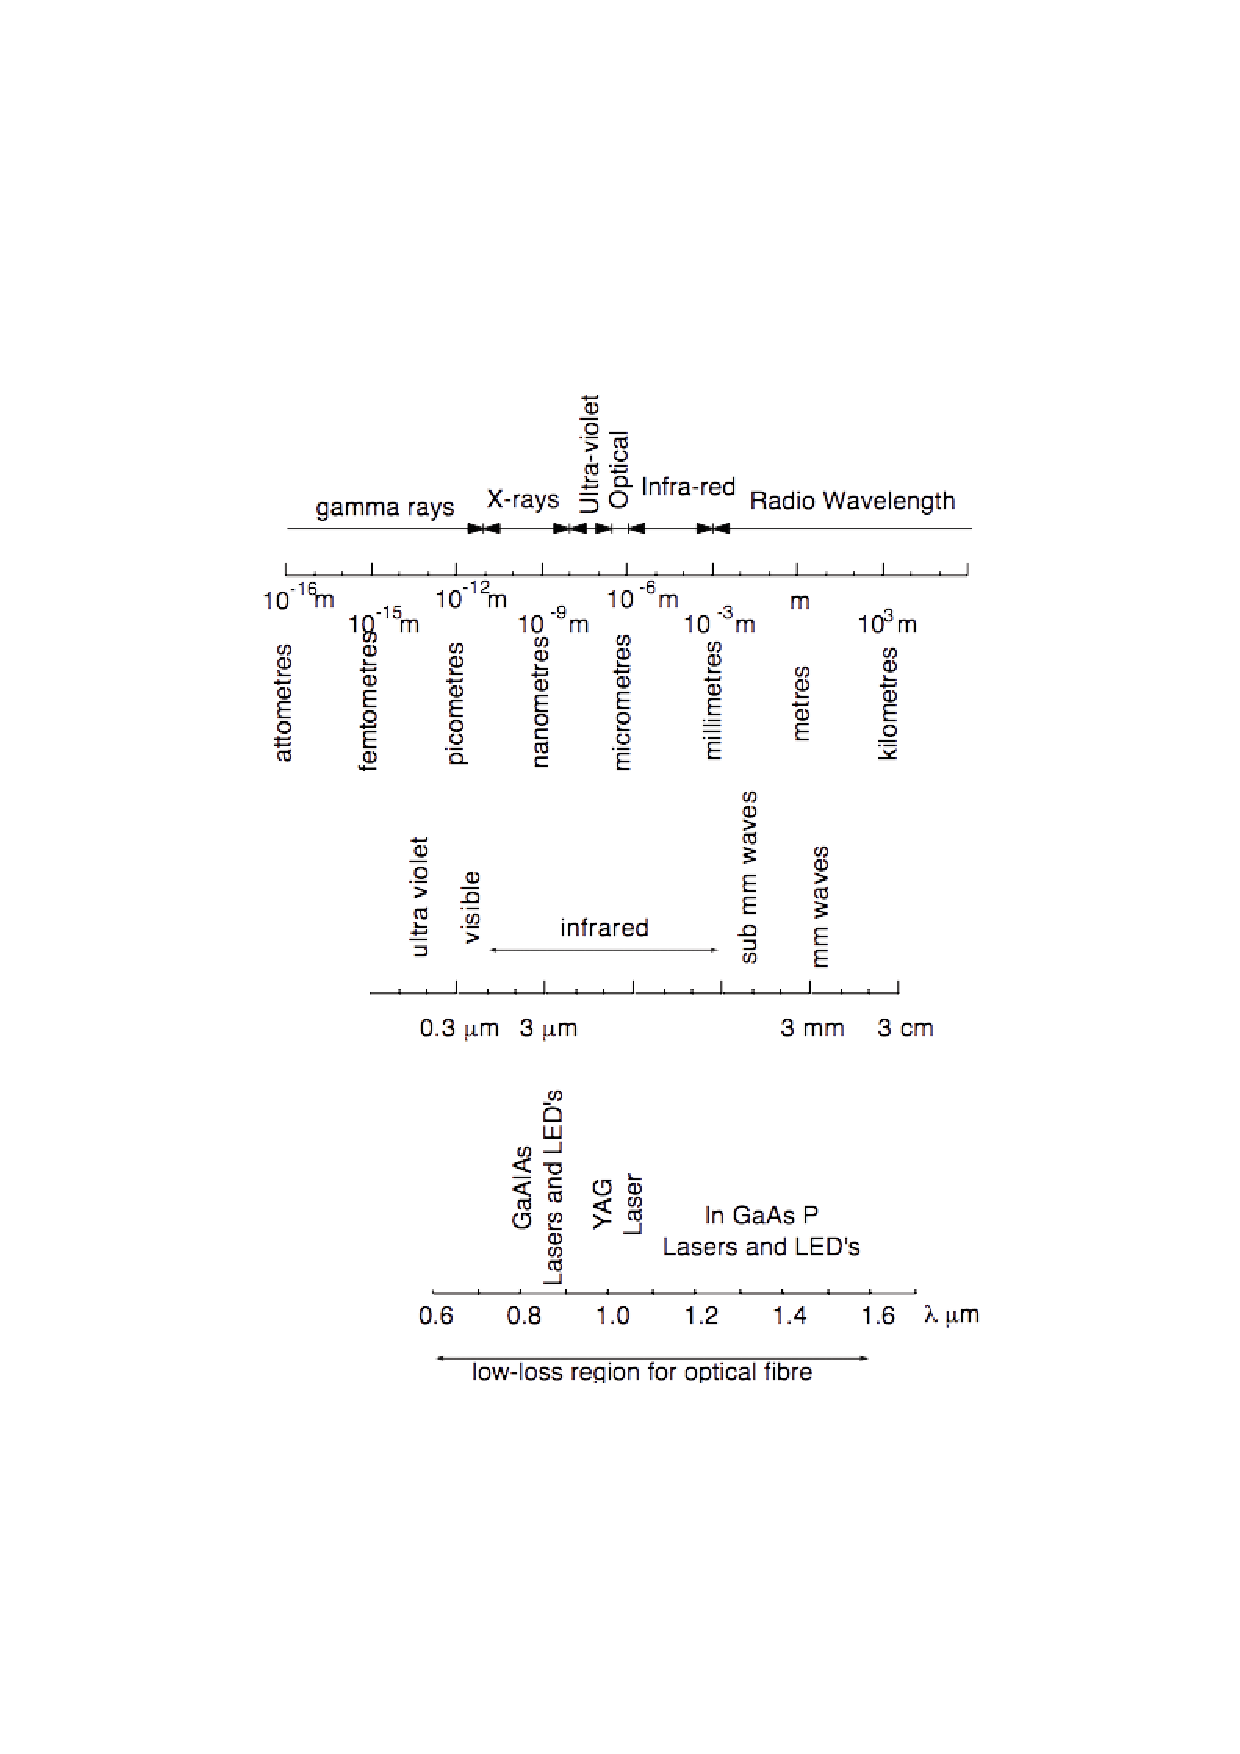
\includegraphics[width=0.75\textwidth]{EMspectrum}}

\def\atmatt{\centering
\includegraphics[width=0.75\textwidth]{atmatt3.eps}}


%



%=========================================================================
\section{Vectors}
%=========================================================================


%=========================================================================
\begin{frame}[fragile]{Vectors}
%
A \alert{linear space} is one upon which addition and scalar multiplication are defined. 

Although such a space is often called a ``vector space'', we will use the term \alert{``vector'' for the geometric concept of a directed line segment}. 

A \alert{\emph{vector}} is a quantity having both \alert{direction and magnitude} in space. 

Examples of vector quantities are force, velocity, acceleration, etc.

We require \alert{linearity}, so that for any vectors $\bf a$ and $\bf b$ we must be able to define their vector sum $ \bf a + b$. 

We define \alert{the product of a scalar $\alpha$ and a vector  $\bf a$} as $\alpha {\bf a}$. The multiplication of a vector times a scalar leaves the direction unchanged and the resulting vector is simply with a different magnitude.


\end{frame}

\section{Inner product}
%=========================================================================
\begin{frame}[shrink=10]{Inner product}
In order to express algebraically the geometric idea of magnitude, it is convenient to define an \alert{Inner product}.

%
\begin{figure}[tb]
\centering
\includegraphics[width=0.25\textwidth]{Dot_Product.png}
\caption{Inner product.}
\label{Dot_Product} 
\end{figure}

The \emph{inner product} ${\bf a} \cdot {\bf b}$
\be
{\bf a} \cdot {\bf b} = \abs{\bf a} \abs{\bf b} \cos \theta
\label{innerp}
\ee
 is the scalar product of two vectors $\bf a$ and $\bf b$ and is a scalar with magnitude $\abs{\bf a} \abs{\bf b} \cos \theta$, where $\abs{\bf a}$ and $\abs{\bf b}$ are the
 lengths of the vectors, and $\theta$ is the angle between them. 
\end{frame}
%%=========================================================================
\begin{frame}[fragile]{Cross product}
%
The \emph{cross product} ${\bf a} \times {\bf b}$ of two vectors is
\be
{\bf a} \times {\bf b} = \abs{\bf a} \abs{\bf b} \sin \theta
\label{outerp}
\ee
i.e. a vector of magnitude $\abs{\bf a} \abs{\bf b} \sin \theta$ in the direction perpendicular to $\bf a$ and $\bf b$, such that \alert{$\bf a$, $\bf b$ and ${\bf a} \times {\bf b}$  form a right-handed set}.

However, \alert{the vector cross product exists only in our 3-dimensional world}; in two dimensions there is simply no direction perpendicular to $\bf a$ and $\bf b$, and in four or more dimensions that direction is ambiguous. 

A more general concept is needed, so that full information about relative directions can still be encoded in all dimensions.
Before introducing the external product we would like to summarize the vector identities. 
\end{frame}

%=========================================================================
\section{Vector identities}
%%=========================================================================
%
\begin{frame}[fragile]{Vector identities}
%


A summary of the vector identities is given in the following

\bea
a & = &  \sqrt{{\bf a} \cdot {\bf a}}  \\
{\bf a} + {\bf b} & = & {\bf b}+ {\bf a}  \\
{\bf a} \cdot {\bf b} & = & {\bf b} \cdot {\bf a}   \label{commutative}\\
{\bf a} \times {\bf b} & = & - {\bf b} \times {\bf a} \label{anticommutative} \\
({\bf a} + {\bf b}) \cdot {\bf c} & = & {\bf a} \cdot {\bf c} +  {\bf b} \cdot {\bf c}   \label{distributive} \\
{\bf a} \cdot {\bf b} \times  {\bf c} & = &  {\bf b}  \cdot  {\bf c} \times {\bf a} =  {\bf c}  \cdot  {\bf a}   \times {\bf b} \label{puntocroce} \\
{\bf a} \times ( {\bf b} \times  {\bf c}) & = &  ({\bf a}  \cdot  {\bf c})  {\bf b} -  ({\bf a}  \cdot  {\bf b})    {\bf c} \label{bacmcab}
\eea
%

\end{frame}
%%=========================================================================
\begin{frame}[fragile]{}
%
Equation (\ref{commutative}) is called the \emph{commutative law}

 while (\ref{distributive}) is the \emph{distributive law}.
 
It is seen from (\ref{anticommutative}) that the cross product is \emph{anticommutative}. 

In (\ref{puntocroce}) it is stated that it is possible to exchange the dot with the cross (naturally the cross product has to be performed first).

In the last equation (\ref{bacmcab}) it is reported a well known identity (often memorized as bac minus cab).

\end{frame}
%%=========================================================================
\begin{frame}[fragile]{}
%
It is noted that the above expressions are \alert{independent from the coordinate system}. If one identity is proved in a coordinate system, it is valid in all the coordinate systems.

\alert{Computation of vector expression may often become quite tedious} and it is of considerable advantage to be able to perform such computations, either symbolically and numerically, with a computer algebra system.

\end{frame}
%
%

%%%=========================================================================
%\begin{frame}[shrink=40]{}
%
%The  code clf.wxm computes wavelength from frequency.
%% The file 
%%\small
%%\begin{verbatim}
%%clf.wxm
%%\end{verbatim}
%%\normalsize
%%
%%is listed in the following.
%
%\small
%\lstinputlisting{clf.wxm}
%\normalsize
%
%
%\end{frame}

\section{Vector identities with Computer Algebra Systems }

%=========================================================================
\begin{frame}[fragile]{}
%
Several Computer Algebra Systems (CAS) are presently available. 

In the following we will make use of \alert{\emph{wxMaxima}} for three reasons: 
%
\begin{itemize}
\item it is freely available; 
\item it runs on several operating systems, 
\item it allows to copy the result as a {\LaTeX}  expression. 
\end{itemize}
%
%We will write simple lines of code that can be cut and past in a  \emph{wxMaxima} window and are ready to run. 
%
The first example will refer to  a segment of code for performing the dot and cross product. The file is: 
%vectors underline v02.wxm.
%%\small
\begin{verbatim}
vectors_v02.wxm
\end{verbatim}
%%\normalsize
%
%%is listed in the following.
%
%\small

%\normalsize
\end{frame}
%%=========================================================================
\begin{frame}[shrink=70]{}
%
\lstinputlisting{vectors_v02.wxm}
\end{frame}
%%=========================================================================
%\begin{frame}[fragile]{}
%
%\end{frame}
%%=========================================================================
%\begin{frame}[fragile]{}
%
%\end{frame}
%%=========================================================================
%\begin{frame}[fragile]{}
%
%\end{frame}
%%=========================================================================
%\begin{frame}[fragile]{}
%
%\end{frame}
%




\end{document}
